\pagestyle{hedra}
\label{hedra}

\begin{textblock*}{5.625in}(0pt,0pt)%
\vspace*{-1.45cm}
\hspace*{-1.8cm}\includegraphics*[width=112mm]{./imgs/HEDRA.png}
\end{textblock*}

\pagebreak


\hspace{.5cm}

\begin{center}
\hspace*{-2.5cm}\raisebox{5.8cm}{\rotatebox[origin=t]{90}{\Formular{\textbf{Lançamento}}}}
\hspace*{2cm}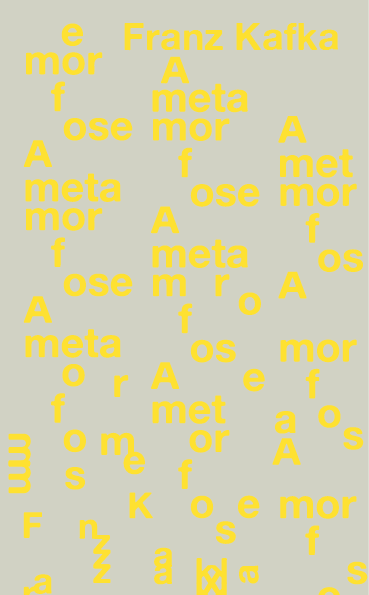
\includegraphics[width=45mm]{./imgs/kafka.png}
\end{center}

\hspace*{-7cm}\hrulefill\hspace*{-7cm}

\medskip

\noindent{}Obra mais famosa de Franz Kafka, {\slsc{A metamorfose}} dispensa apresentações. A história da transformação de Gregor Samsa é um clássico porque condensa perfeitamente as características da prosa kafkiana, este conceito que se torna importante na nossa repertoriação do mundo: kafkiano é, pois, o contraditório da nossa cultura ocidental desumanizada, em que o irracional é criado justamente pelas estruturas burocráticas ultrarracionalizadas.

%\hspace{.5cm}
\vfill

\hspace*{-.4cm}\begin{minipage}[c]{1\linewidth}
\small{
{\Formular{\textbf{
\hspace*{-.1cm}Título: A metamorfose\\
Autor: Franz Kafka\\ 
Editora: Hedra\\
Páginas: 196\\
Formato: 13x21cm\\
Preço: R\$ 39,90\\
ISBN: 978-85-7715-601-6
}}}}
\end{minipage}


\pagebreak

\hspace{.5cm}

\begin{center}
\hspace*{-.5cm}
\includegraphics[width=45mm]{./imgs/maquiavel.png}
\end{center}

\hspace*{-7cm}\hrulefill\hspace*{-7cm}

\medskip

\noindent{}{\slsc{O príncipe}} ganha sua mais completa edição bilíngue, trazendo ao leitor brasileiro contato com a melhor edição do texto original italiano --- a Edição Crítica Inglese ---, acrescida de introdução e notas explicativas. Obra mais emblemática de Nicolau Maquiavel, {\slsc{O príncipe}} assinala uma nova forma de analisar a política, marcada principalmente pelo realismo que procura apreender a política como ela é --- em sua prática terrena.

%\hspace{.5cm}
\vfill

\hspace*{-.4cm}\begin{minipage}[c]{1\linewidth}
\small{
{\Formular{\textbf{
\hspace*{-.1cm}Título: O príncipe\\
Autor: Nicolau Maquiavel\\ 
Editora: Hedra\\
Páginas: 508\\
Formato: 13x21cm\\
Preço: R\$ 49,90\\
ISBN: 978-85-7715-604-7
}}}}
\end{minipage}

\pagebreak

\hspace{.5cm}

\begin{center}
\hspace*{-2.7cm}\raisebox{5.5cm}{\rotatebox[origin=t]{90}{\Formular{\textbf{Lançamento}}}}
\hspace*{2cm}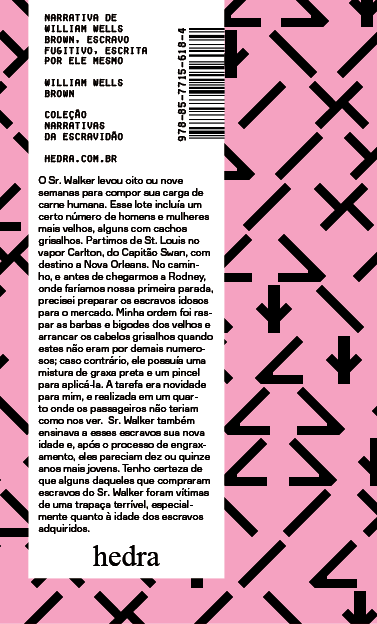
\includegraphics[width=43mm]{./imgs/wwb.png}
\end{center}

\hspace*{-7cm}\hrulefill\hspace*{-7cm}

\medskip

\noindent{}Romancista, dramaturgo, historiador e militante abolicionista, William Wells Brown tem em sua {\slsc{Narrativa autobiográfica}} um dos mais importantes romances afro"-americanos da história. A obra reconta os horrores da escravidão, percorrendo o tráfico interno de escravos nos \scalebox{.8}{EUA} e a relação de Brown com seus donos e familiares, destacando assim a individualidade e que se desenvolveu sob uma instituição totalizante e desumanizadora.

%\hspace{.5cm}
\vfill

\hspace*{-.4cm}\begin{minipage}[c]{1\linewidth}
\small{
{\Formular{\textbf{
\hspace*{-.1cm}Título: Narrativa de William Wells Brown, escravo fugitivo, escrita por ele mesmo\\
Autor: William Wells Brown\\ 
Editora: Hedra\\
Páginas: 142\\
Formato: 14x21cm\\
Preço: R\$ 39,90\\
ISBN: 978-85-7715-618-4
}}}}
\end{minipage}

\pagebreak

\hspace{.5cm}

\begin{center}
\hspace*{-.5cm}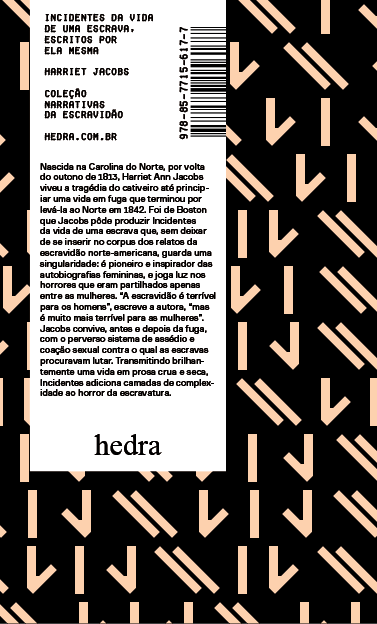
\includegraphics[width=43mm]{./imgs/jacobs.png}
\end{center}

\hspace*{-7cm}\hrulefill\hspace*{-7cm}

\medskip

\noindent{}Nascida na Carolina do Norte, por volta do outono de 1813, Harriet Ann Jacobs viveu intensamente a tragédia da escravidão, e dela resulta este relato cru, de prosa vívida e dramática que, sem deixar de se inserir no corpus dos relatos da escravidão norte"-americana, é pioneiro e inspirador das autobiografias femininas, e joga luz no perverso sistema de assédio e coação que era partilhado apenas entre as mulheres.

%\hspace{.5cm}
\vfill

\hspace*{-.4cm}\begin{minipage}[c]{1\linewidth}
\small{
{\Formular{\textbf{
\hspace*{-.1cm}Título: Incidentes da vida de uma escrava, escritos por ela mesma\\
Autor: Harriet Jacobs\\ 
Editora: Hedra\\
Páginas: 406\\
Formato: 14x21cm\\
Preço: R\$ 49,90\\
ISBN: 978-85-7715-617-7
}}}}
\end{minipage}


\pagebreak

\hspace{.5cm}

\begin{center}
\hspace*{-2.7cm}\raisebox{5.5cm}{\rotatebox[origin=t]{90}{\Formular{\textbf{Lançamento}}}}
\hspace*{2cm}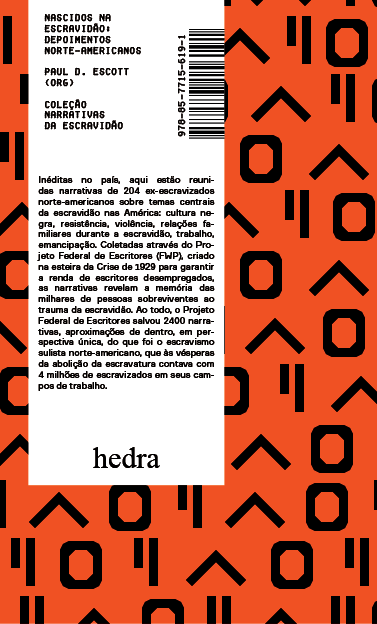
\includegraphics[width=43mm]{./imgs/wpa.png}
\end{center}

\hspace*{-7cm}\hrulefill\hspace*{-7cm}

\medskip

\noindent{}{\slsc{Nascidos na escravidão}} resulta de um amplo esforço de tomar depoimentos de ex"-escravos dos Estados Unidos, totalizando 2400 narrativas inéditas, das quais a edição reúne 204, em uma curadoria por tema que permite entrever a memória das milhares de pessoas sobreviventes do trauma do cativeiro, em sua complexidade, e desmontar certos mitos correntes sobre a escravidão através de depoimentos em primeira mão.


%\hspace{.5cm}
\vfill

\hspace*{-.4cm}\begin{minipage}[c]{1\linewidth}
\small{
{\Formular{\textbf{
\hspace*{-.1cm}Título: Nascidos na escravidão: depoimentos norte"-americanos\\
Autor: Paul D. Scott (org.)\\ 
Editora: Hedra\\
Páginas: 348\\
Formato: 14x21cm\\
Preço: R\$ 49,90\\
ISBN: 978-85-7715-619-1
}}}}
\end{minipage}

\pagebreak

\hspace{.5cm}

\begin{center}
\hspace*{-.5cm}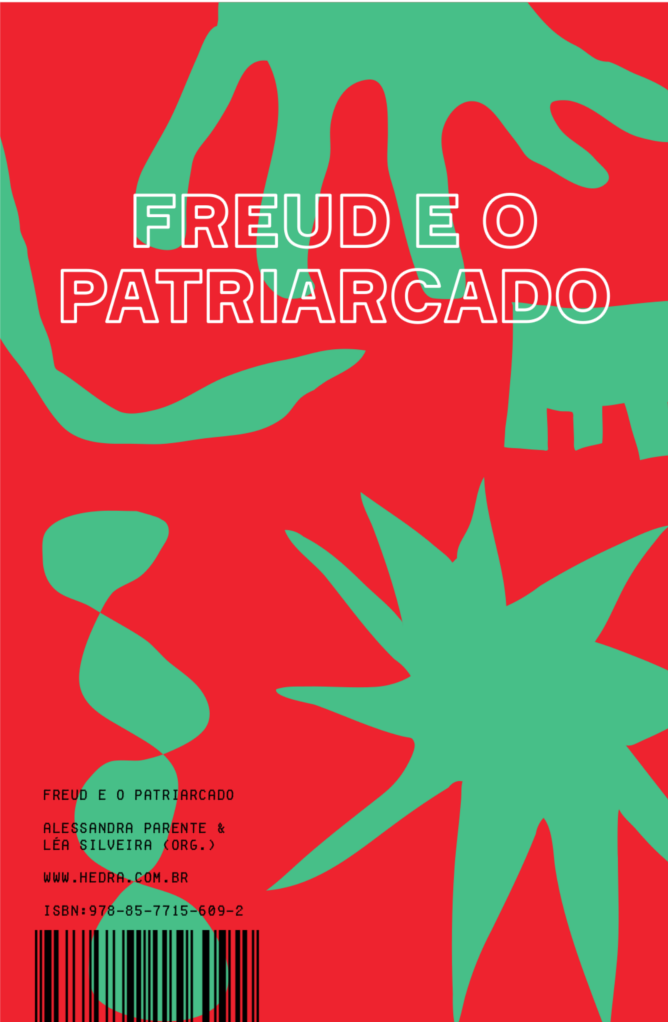
\includegraphics[width=46.5mm]{./imgs/freud.png}
\end{center}

\hspace*{-7cm}\hrulefill\hspace*{-7cm}

\medskip

\noindent{}{\slsc{Freud e o patriarcado}} parte da constatação de que o campo da teoria psicanalítica põe em jogo uma forma de conceber o psíquico que assume, em seu centro, uma equivalência generalizada entre cultura, civilização e masculinidade, algo que, para as autoras e os autores de {\slsc{Freud e o patriarcado}}, deveria ser explicado, não dado. Sobre essa trilha, trata"-se de explorar a legitimidade dos modelos freudianos, seja preservando"-os ou repensando"-os.

%\hspace{.5cm}
\vfill

\hspace*{-.4cm}\begin{minipage}[c]{1\linewidth}
\small{
{\Formular{\textbf{
\hspace*{-.1cm}Título: Freud e o patriarcado\\
Autor: Alessandra Martins Parente e Léa Silveira (org.)\\ 
Editora: Hedra\\
Páginas: 398\\
Formato: 16x23cm\\
Preço: R\$ 64,90\\
ISBN: 978-85-7715-611-5
}}}}
\end{minipage}

\pagebreak

\hspace{.5cm}

\begin{center}
\hspace*{-1cm}\raisebox{5.5cm}{\rotatebox[origin=t]{90}{\Formular{\textbf{Lançamento}}}}
\hspace*{1cm}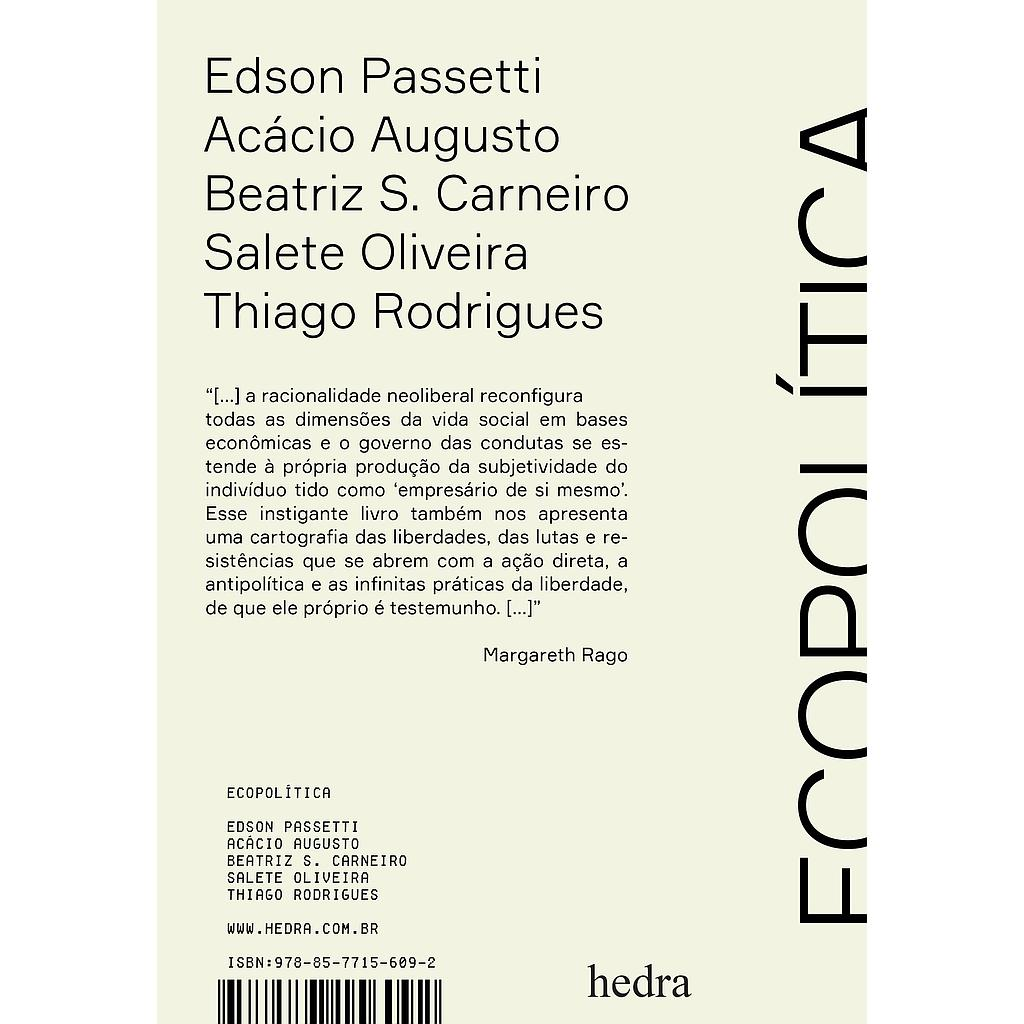
\includegraphics[width=70mm]{./eco.jpeg}
\end{center}

\hspace*{-7cm}\hrulefill\hspace*{-7cm}

\medskip

\noindent{}{\slsc{Ecopolítica}} mapeia a passagem da biopolítica — o controle da vida analisado por Foucault — para a ecopolítica, nova forma de governar que emerge pós-\scalebox{.8}{II} Guerra Mundial e se estende a todas as esferas do mundo natural. Os estudiosos do grupo Nu"-Sol percorrem e analisam acontecimentos históricos e contemporâneos, e atravessam fluxos de poder para conclamar à criação de resistências libertárias e esquivas às globalizantes linhas de controle.

%\hspace{.5cm}
\vfill

\hspace*{-.4cm}\begin{minipage}[c]{1\linewidth}
\small{
{\Formular{\textbf{
\hspace*{-.1cm}Título: Ecopolítica\\
Autor: Edson Passetti (org.)\\ 
Editora: Hedra\\
Páginas: 476\\
Formato: 16x23cm\\
Preço: R\$ 79,90\\
ISBN: 978-85-7715-609-2
}}}}
\end{minipage}

\pagebreak

\hspace{.5cm}

\begin{center}
\hspace*{-.5cm}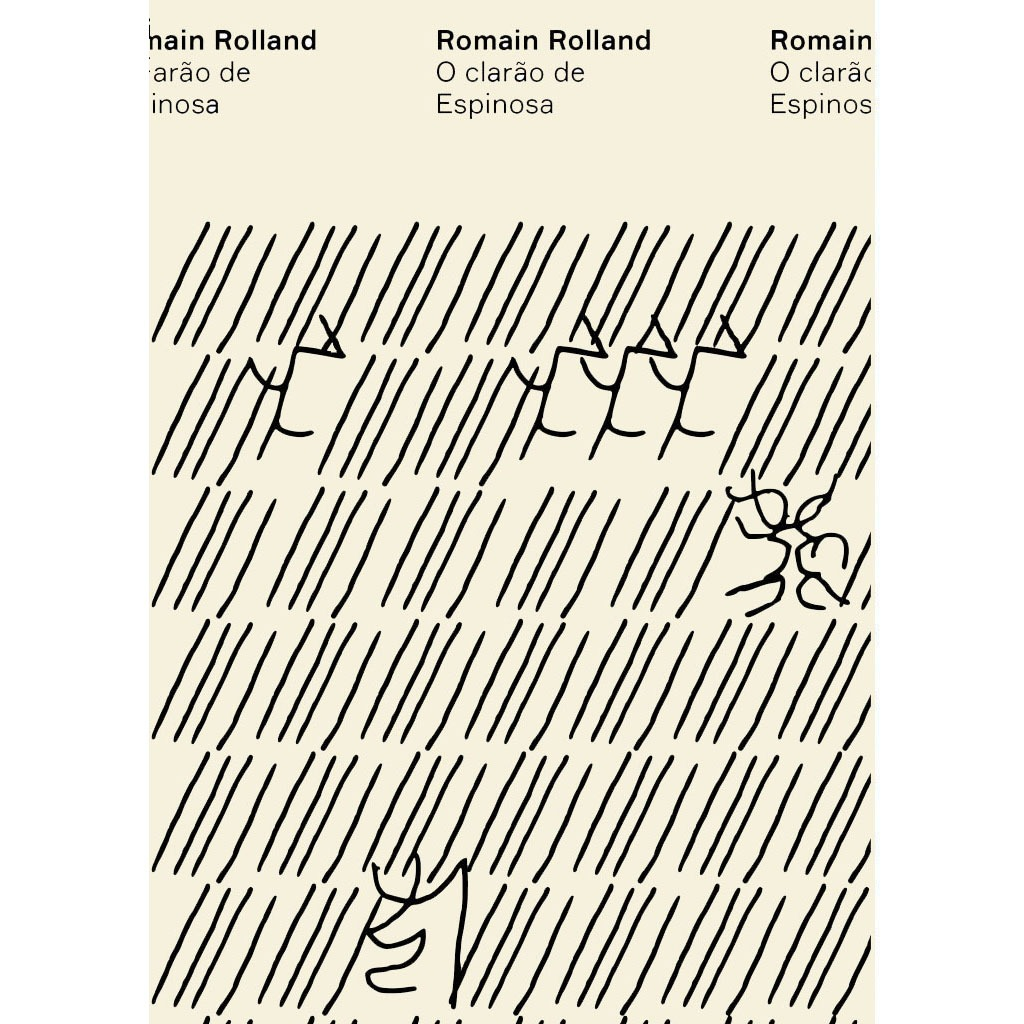
\includegraphics[width=70mm]{./grid/romain.jpeg}
\end{center}

\hspace*{-7cm}\hrulefill\hspace*{-7cm}

\medskip

\noindent{}Romain Rolland (1866-1944) novelista, biógrafo e músico francês (Nobel de 1915) escreveu estas páginas sobre Espinosa, que fazem parte de {\slsc{Confissões inéditas}}, capítulo do livro intitulado {\slsc{A viagem interior}} (1942) . Neste pequeno trecho o adolescente Romain Rolland conta o “clarão” que teve em sua vida ao ler Espinosa pela primeira vez aos 16 anos e como isso definiu sua vida e carreira.

\vfill

\hspace*{-.4cm}\begin{minipage}[c]{1\linewidth}
\small{
{\Formular{\textbf{
\hspace*{-.1cm}Título: O clarão de Espinosa\\
Autor: Romain Rolland\\ 
Editora: n-1 / Hedra\\
Páginas: 57\\
Formato: 11x18cm\\
Preço: R\$ 29,90\\
ISBN: 978-65-8109-708-0
}}}}
\end{minipage}

\pagebreak

\hspace{.5cm}

\begin{center}
\hspace*{-1cm}\raisebox{5.5cm}{\rotatebox[origin=t]{90}{\Formular{\textbf{Lançamento}}}}
\hspace*{1cm}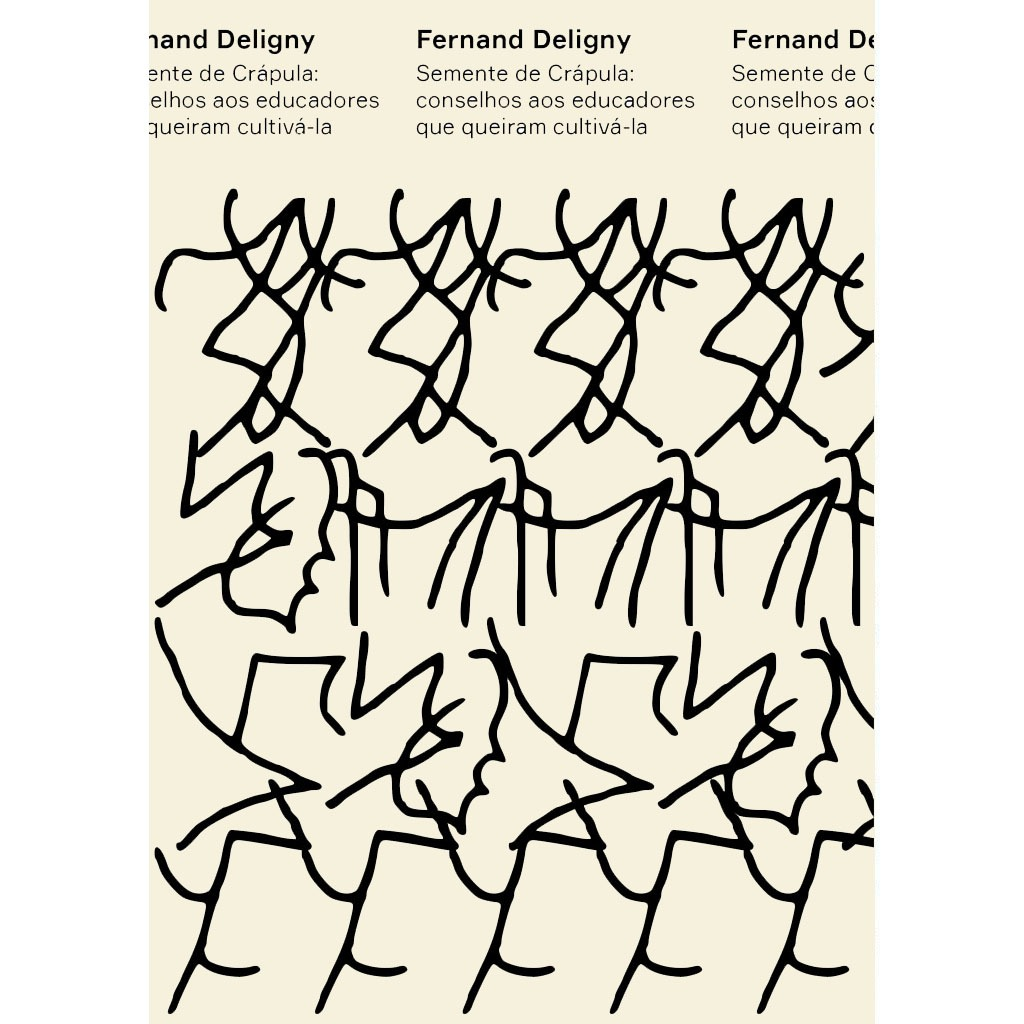
\includegraphics[width=70mm]{./grid/deligny.jpeg}
\end{center}

\hspace*{-7cm}\hrulefill\hspace*{-7cm}

\medskip

\noindent{}{\slsc{Semente de crápula}} é o primeiro livro de Fernand Deligny e um balizador do seu trabalho que o situaria enquanto uma das maiores referências da educação especial. Em belos aforismas, as sementes de que aqui se trata são de jovens, cultivados pelo educador que deve deixar de lutar contra as ervas daninhas, pragas sociais atadas ao nosso convívio social, para mergulhar nas dinâmicas espaciais dos jovens.

\vfill

\hspace*{-.4cm}\begin{minipage}[c]{1\linewidth}
\small{
{\Formular{\textbf{
\hspace*{-.1cm}Título: Semente de crápula: conselhos aos educadores que queiram cultivá-la\\
Autor: Fernand Deligny\\ 
Editora: n-1 / Hedra\\
Páginas: 96\\
Formato: 11x18cm\\
Preço: R\$ 34,90\\
ISBN: 978-65-8109-709-7
}}}}
\end{minipage}

\pagebreak

\hspace{.5cm}

\begin{center}
\hspace*{-.5cm}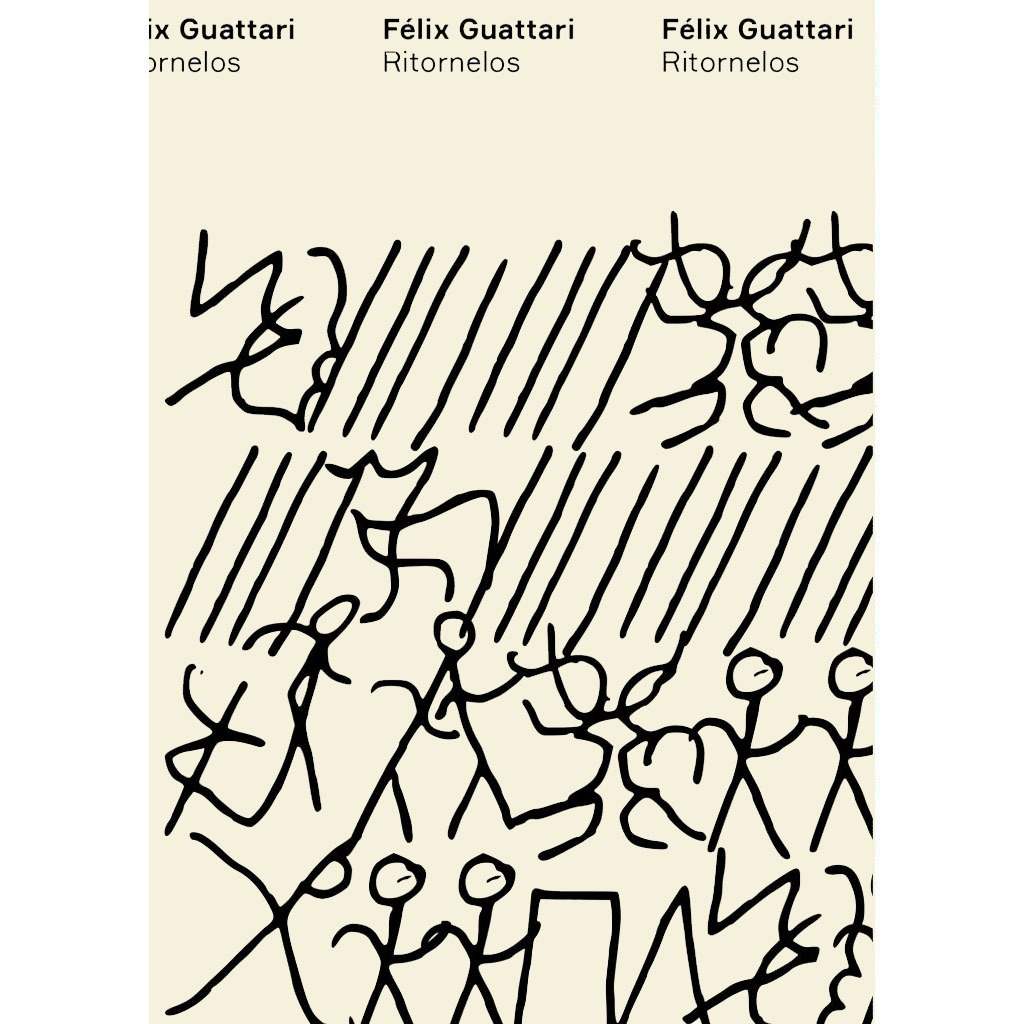
\includegraphics[width=70mm]{./grid/guattari.jpeg}
\end{center}

\hspace*{-7cm}\hrulefill\hspace*{-7cm}

\medskip

\noindent{}Livro póstumo do pensador e psicanalista Félix Guattari, {\slsc{Ritornelos}} é inclassificável. Misto de poesia, relatos autobiográficos, frames do cotidiano, toda potência da escrita esquiza irrompe nessas páginas de alta voltagem poética e imagética. Além de arguto intelectual, Guattari aparece em {\slsc{Ritornelos}} enquanto poeta sensível aos instantâneos e surreais quadros da vida.

\vfill

\hspace*{-.4cm}\begin{minipage}[c]{1\linewidth}
\small{
{\Formular{\textbf{
\hspace*{-.1cm}Título: Ritornelos\\
Autor: Félix Guattari\\ 
Editora: n-1 / Hedra\\
Páginas: 134\\
Formato: 11x18cm\\
Preço: R\$ 40,00\\
ISBN: 978-65-81097-02-8
}}}}
\end{minipage}

\pagebreak

\hspace{.5cm}

\begin{center}
\hspace*{-1cm}\raisebox{5.5cm}{\rotatebox[origin=t]{90}{\Formular{\textbf{Lançamento}}}}
\hspace*{1cm}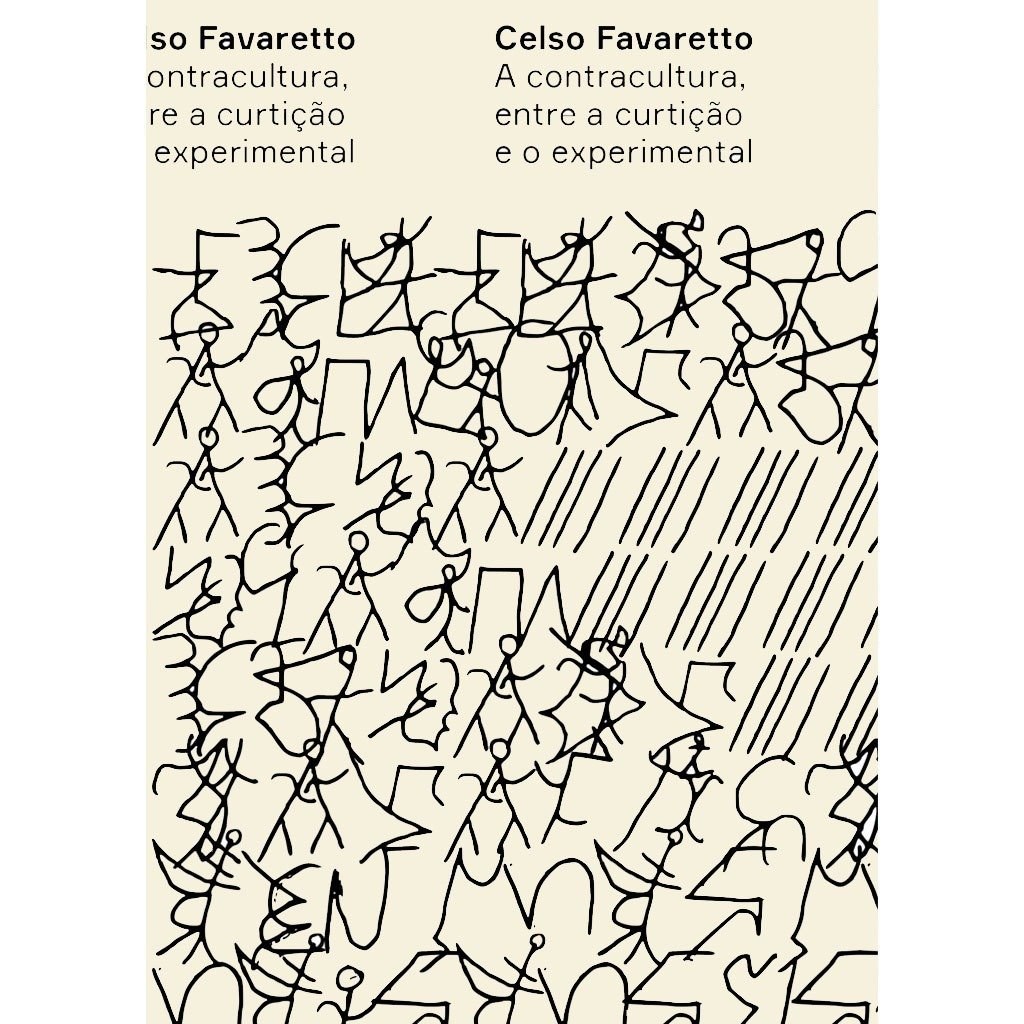
\includegraphics[width=70mm]{./grid/favaretto.jpeg}
\end{center}

\hspace*{-7cm}\hrulefill\hspace*{-7cm}

\medskip

\noindent{}Em {\slsc{Contracultura}}, Celso Favaretto aborda as manifestações que marcaram a produção artística brasileira entre os anos 60 e 70. Manifestava"-se então uma nova sensibilidade, que explorava as possibilidades abertas pelo tropicalismo. Para o autor, longe de um suposto “vazio cultural”, a contracultura, em suas expressões, definiu comportamentos e experimentações de grande vitalidade, inclusive como resistência à cultura oficial e à ditadura.

\vfill

\hspace*{-.4cm}\begin{minipage}[c]{1\linewidth}
\small{
{\Formular{\textbf{
\hspace*{-.1cm}Título: A contracultura, entre a curtição e o experimental\\
Autor: Celso Favaretto\\ 
Editora: n-1 / Hedra\\
Páginas: 142\\
Formato: 11x18cm\\
Preço: R\$ 40,00\\
ISBN: 978-65-81097-03-5 
}}}}
\end{minipage}

\pagebreak